\begin{frame}{}
    \LARGE GAN Variant: \\[1.5ex] \textbf{Wasserstein GANs (WGANs)}
\end{frame}

\begin{frame}[allowframebreaks]{Wasserstein GAN}
\begin{itemize}
    \item Wasserstein GAN uses wasserstein distance instead of crossentropy loss.
    \item Wasserstein distance that has a smoother gradient everywhere.
        \begin{figure}
            \centering
            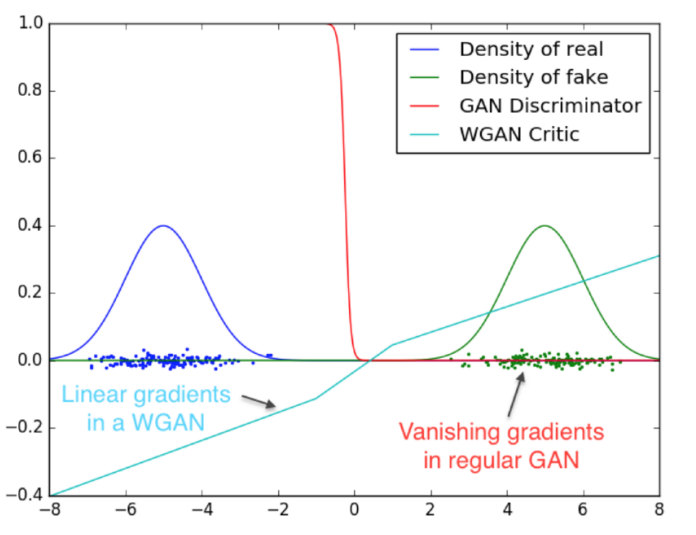
\includegraphics[height=0.6\textheight, width=\textwidth, keepaspectratio]{images/gan/wgan_1.png}
        \end{figure}
\end{itemize}
    
\end{frame}

\begin{frame}{Wasserstein Distance}
\begin{itemize}
    \item Intuitively, it is the shovels of earth moved to make two distributions look alike.
    \begin{figure}
        \centering
        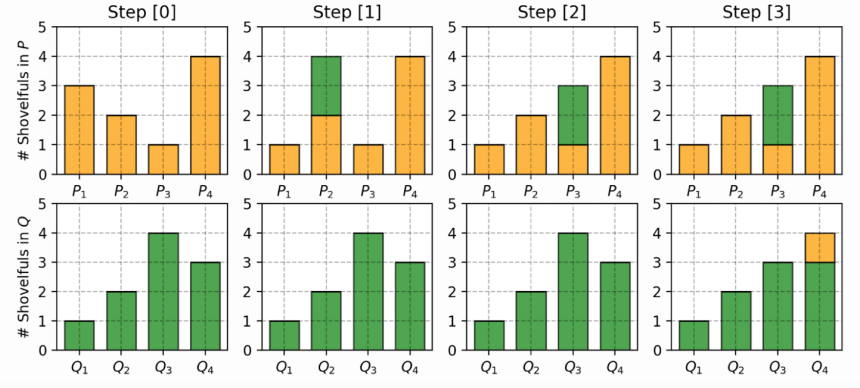
\includegraphics[height=0.6\textheight, width=\textwidth, keepaspectratio]{images/gan/wgan_2.png}
        \caption*{Step by Step plan of moving dirt between piles $P$ and $Q$ to make them match}
    \end{figure}
    
\end{itemize}
    
\end{frame}

\begin{frame}[allowframebreaks]{WGAN}
\begin{figure}
    \centering
    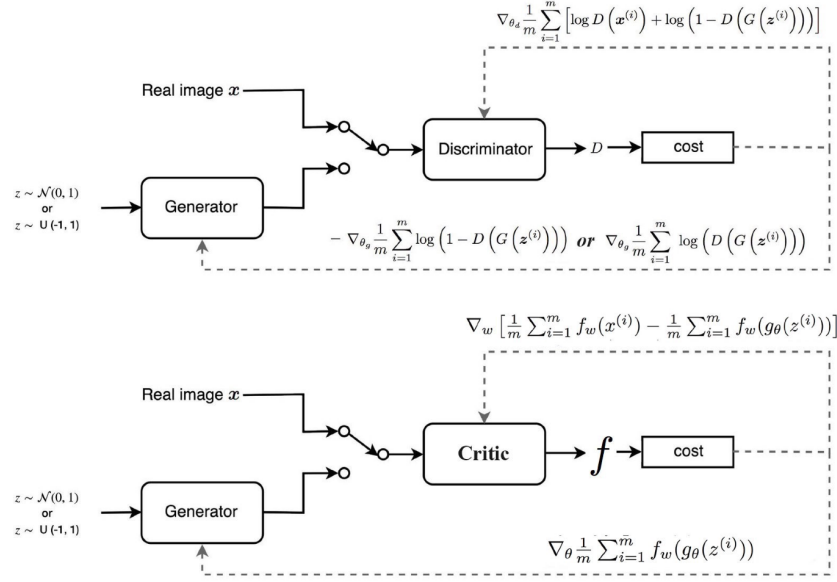
\includegraphics[height=0.9\textheight, width=\textwidth, keepaspectratio]{images/gan/wgan_3.png}
\end{figure}

\framebreak
\begin{figure}
    \centering
    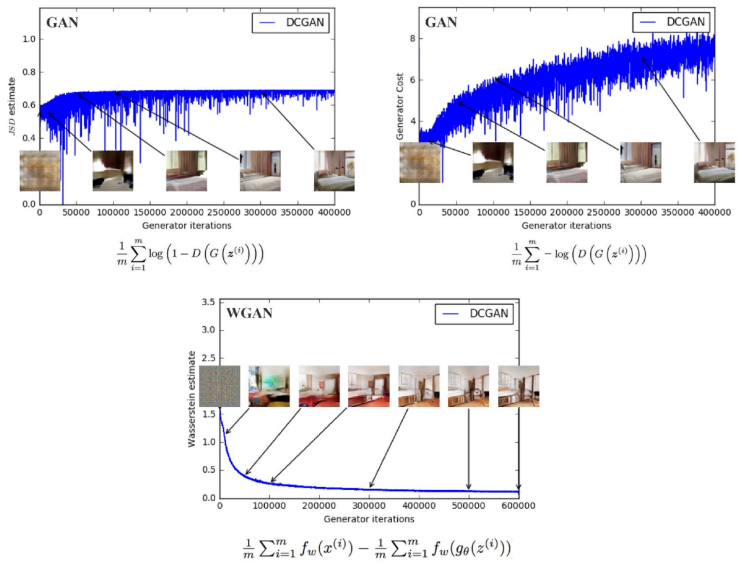
\includegraphics[height=0.9\textheight, width=\textwidth, keepaspectratio]{images/gan/wgan_4.png}
\end{figure}

\framebreak
\begin{figure}
    \centering
    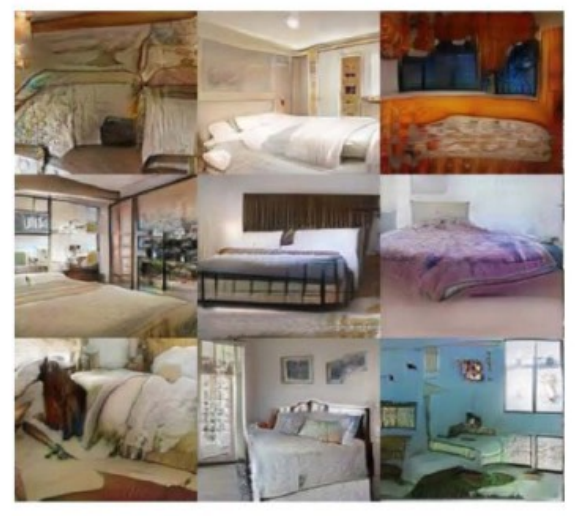
\includegraphics[height=0.8\textheight, width=\textwidth, keepaspectratio]{images/gan/wgan_5.png}
    \caption*{WGAN generation results on bedroom images}
\end{figure}

\end{frame}

\begin{frame}[allowframebreaks]{WGAN-GP: Gradient Penalty for Lipschitzness}
\begin{figure}
    \centering
    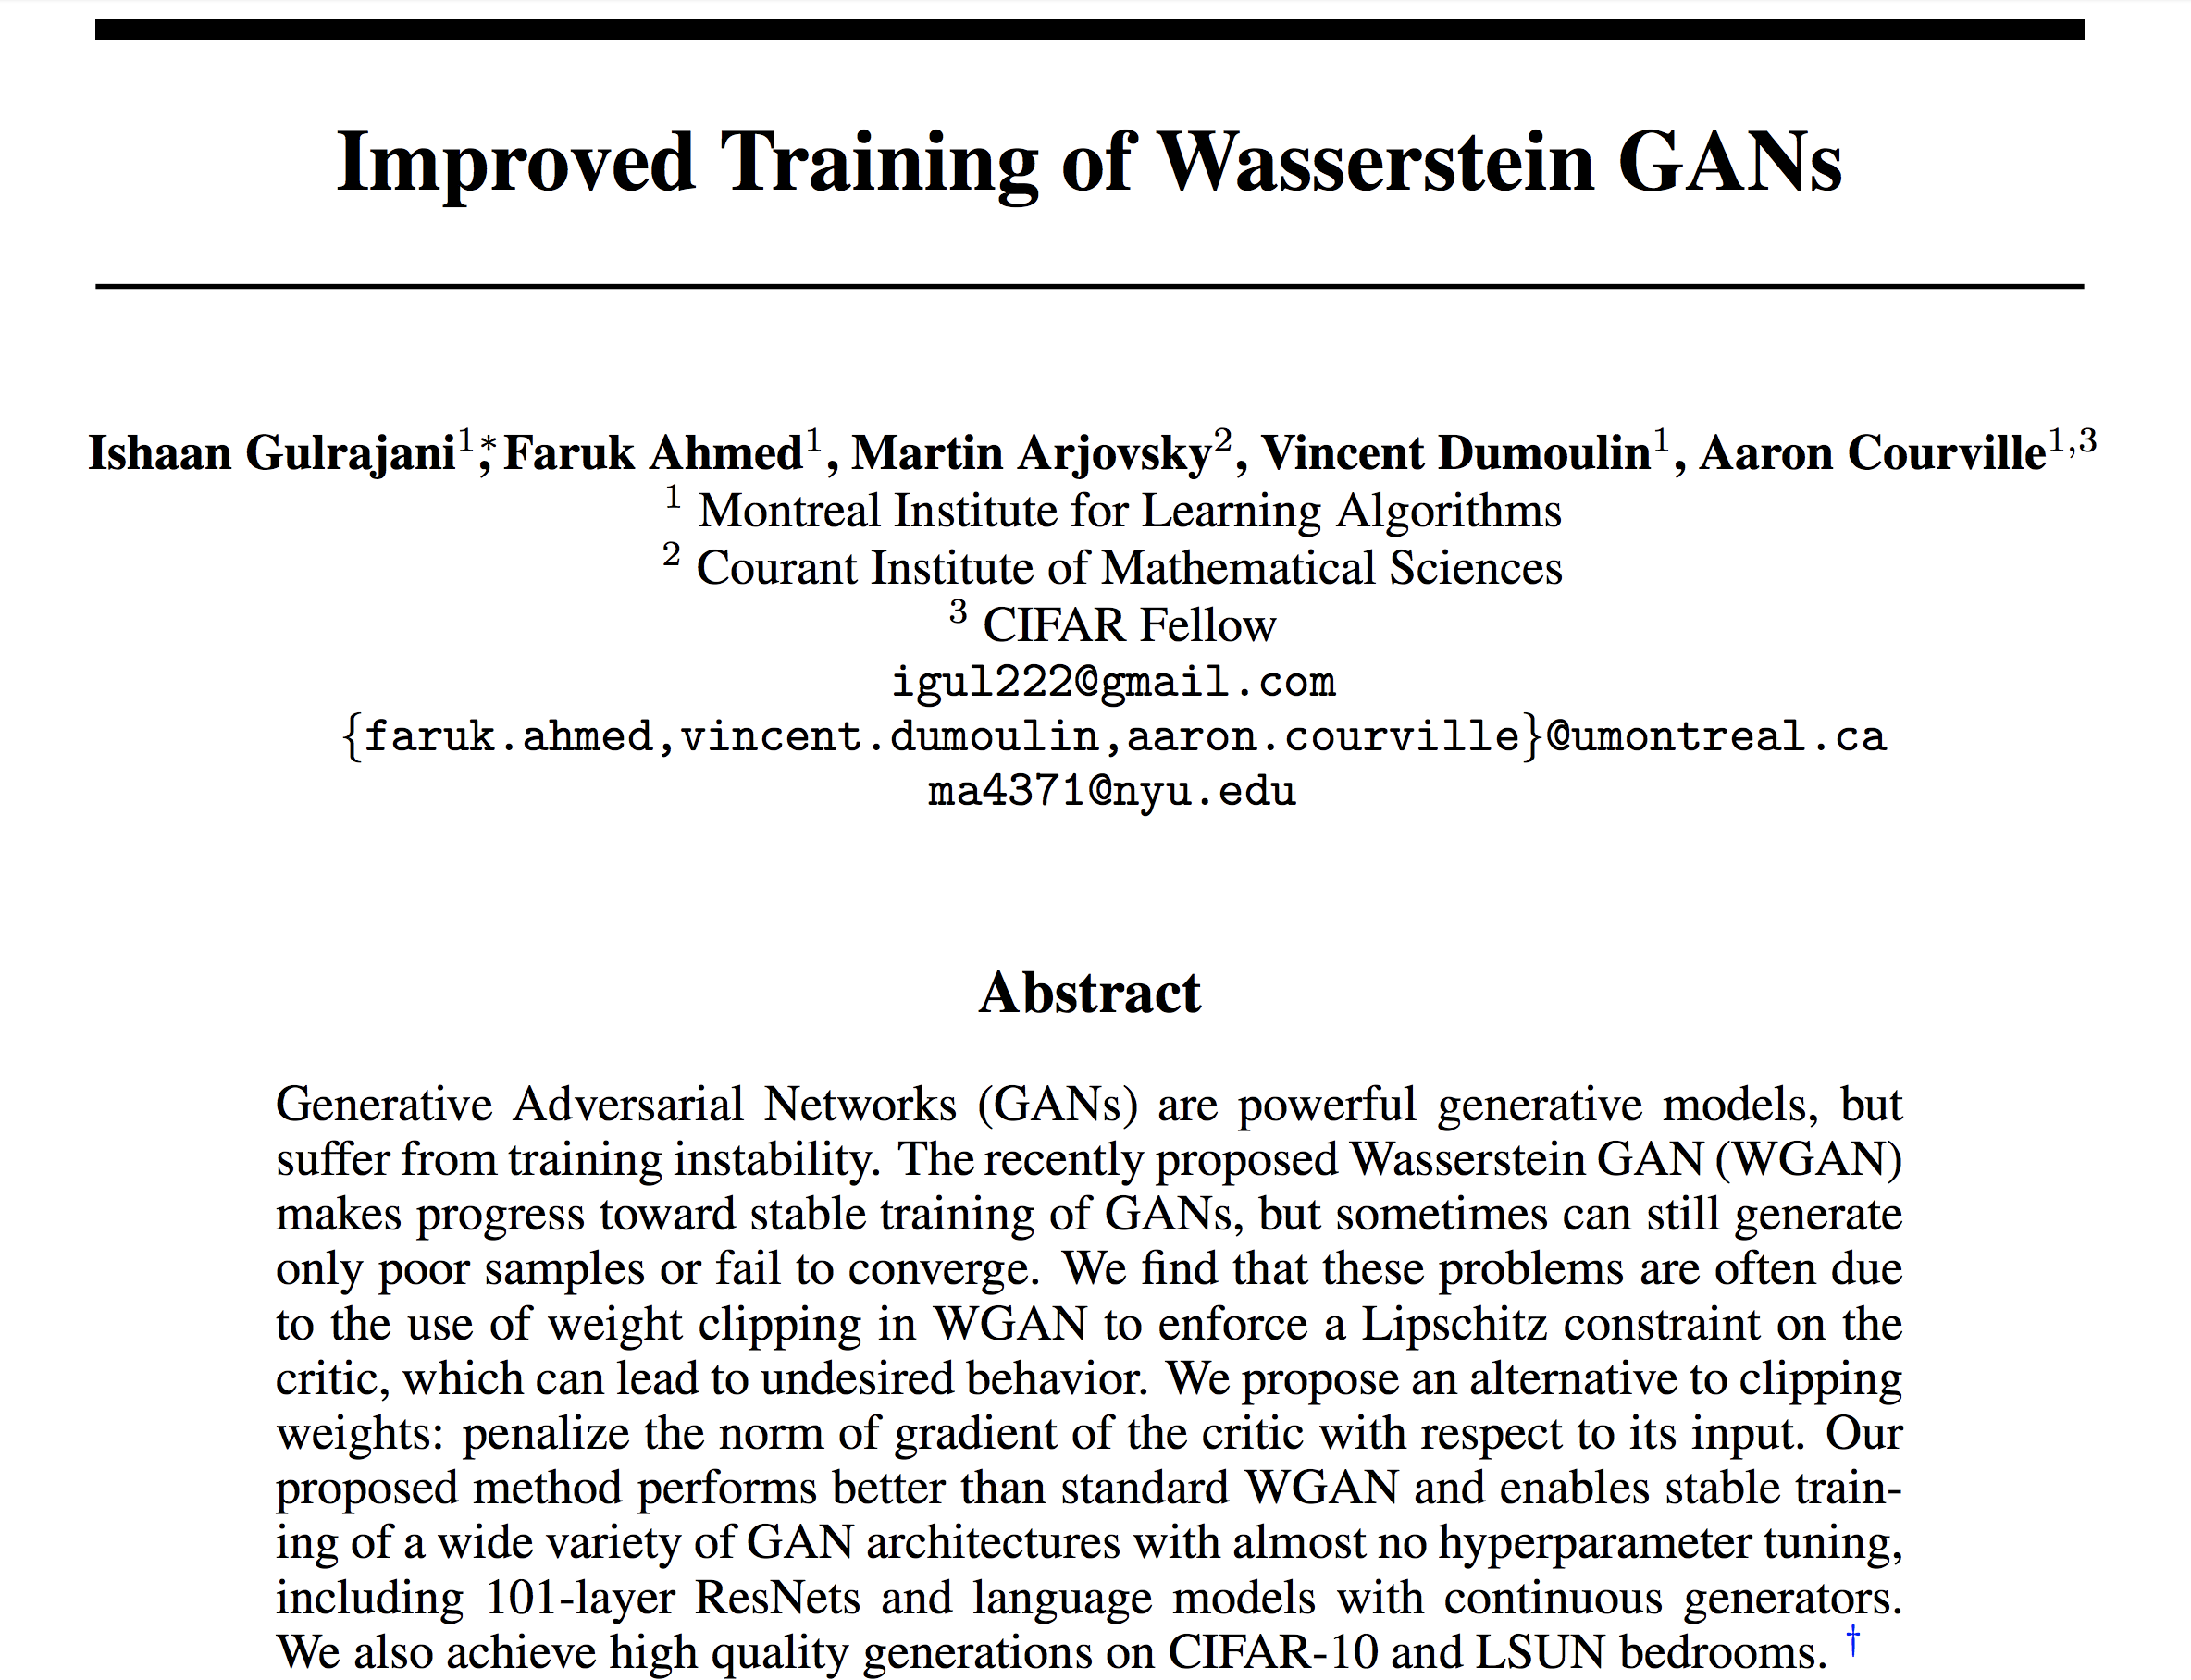
\includegraphics[height=0.8\textheight, width=\textwidth, keepaspectratio]{images/gan/wgan-gp/slide_84_1_img.png}
    \caption*{[Gulrajani et al 2017]}
\end{figure}

\framebreak
\begin{columns}
    \column{0.6\textwidth}
    \begin{figure}
        \centering
        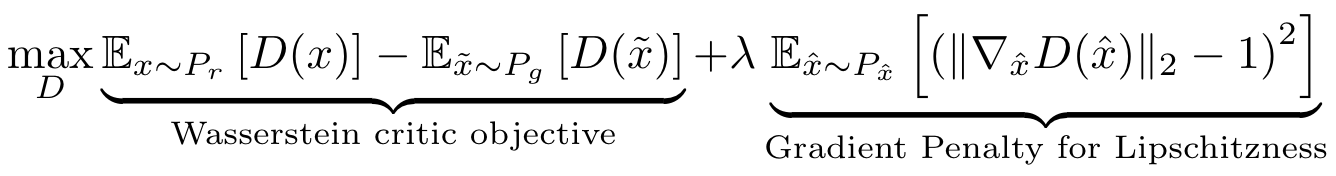
\includegraphics[height=0.8\textheight, width=\textwidth, keepaspectratio]{images/gan/wgan-gp/slide_85_3_img.png}
    \end{figure}
    \begin{figure}
        \centering
        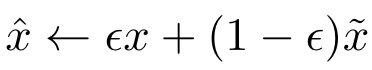
\includegraphics[height=0.1\textheight, width=\textwidth, keepaspectratio]{images/gan/wgan-gp/slide_85_4_img.png}
    \end{figure}
    \column{0.5\textwidth}
    \begin{figure}
        \centering
        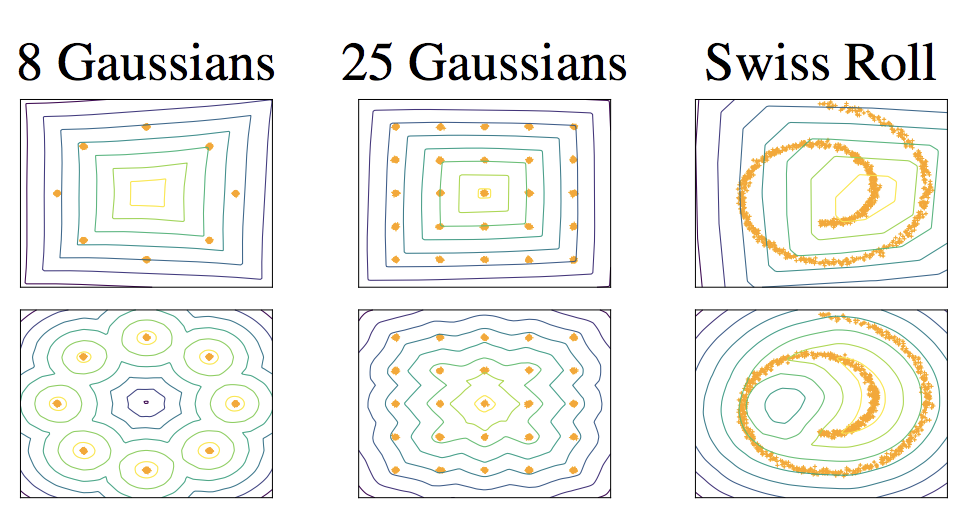
\includegraphics[height=0.8\textheight, width=1.05\textwidth, keepaspectratio]{images/gan/wgan-gp/slide_85_2_img.png}
    \end{figure}
    \begin{figure}
        \centering
        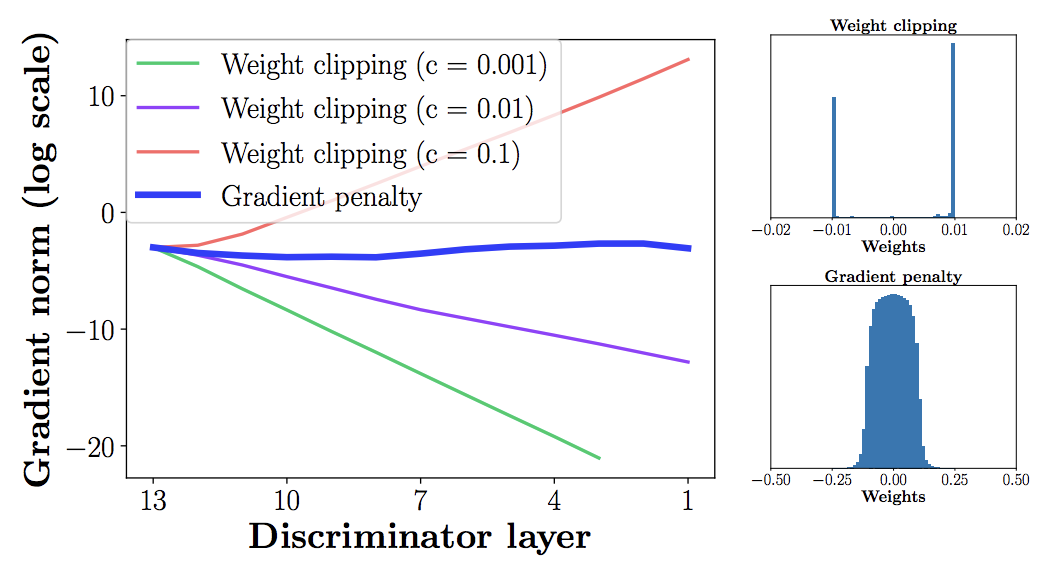
\includegraphics[height=0.8\textheight, width=1.05\textwidth, keepaspectratio]{images/gan/wgan-gp/slide_85_1_img.png}
    \end{figure}
\end{columns}
\end{frame}

\begin{frame}[allowframebreaks]{WGAN-GP: Pseudocode}
    \begin{figure}
        \centering
        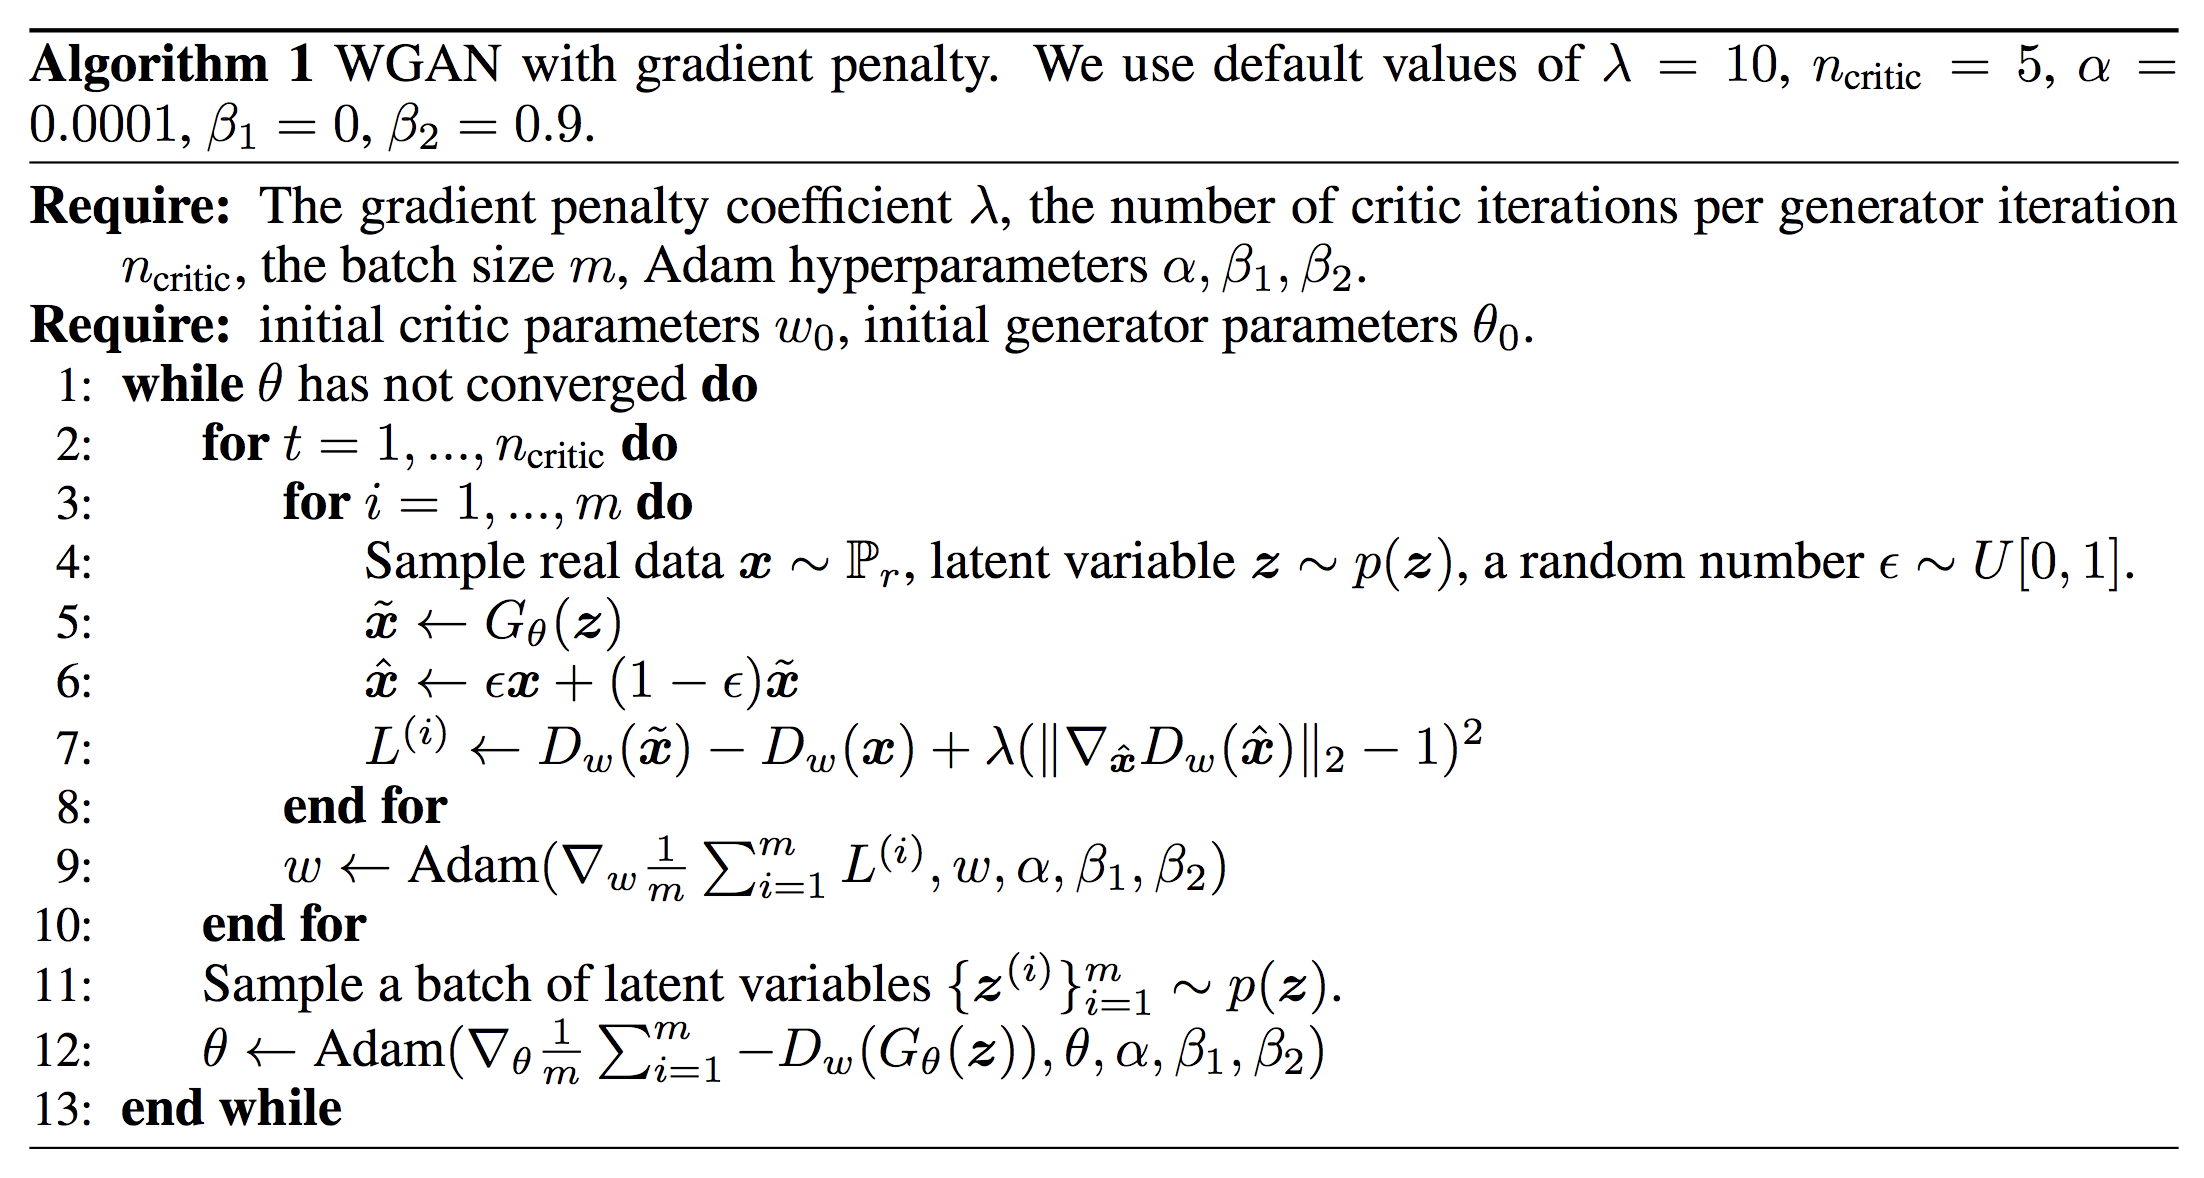
\includegraphics[height=0.8\textheight, width=1.05\textwidth, keepaspectratio]{images/gan/wgan-gp/slide_86_1_img.png}
        \caption*{[Gulrajani et al 2017]}
    \end{figure}
\end{frame}

\begin{frame}[allowframebreaks]{WGAN-GP: BatchNorm}
    \begin{figure}
        \centering
        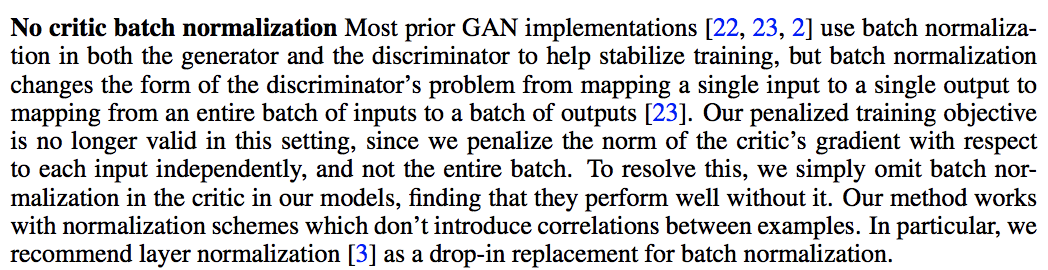
\includegraphics[height=0.8\textheight, width=1.05\textwidth, keepaspectratio]{images/gan/wgan-gp/slide_87_1_img.png}
        \caption*{[Gulrajani et al 2017]}
    \end{figure}
\end{frame}

\begin{frame}[allowframebreaks]{WGAN-GP: Robustness to architectures}
    \begin{figure}
        \centering
        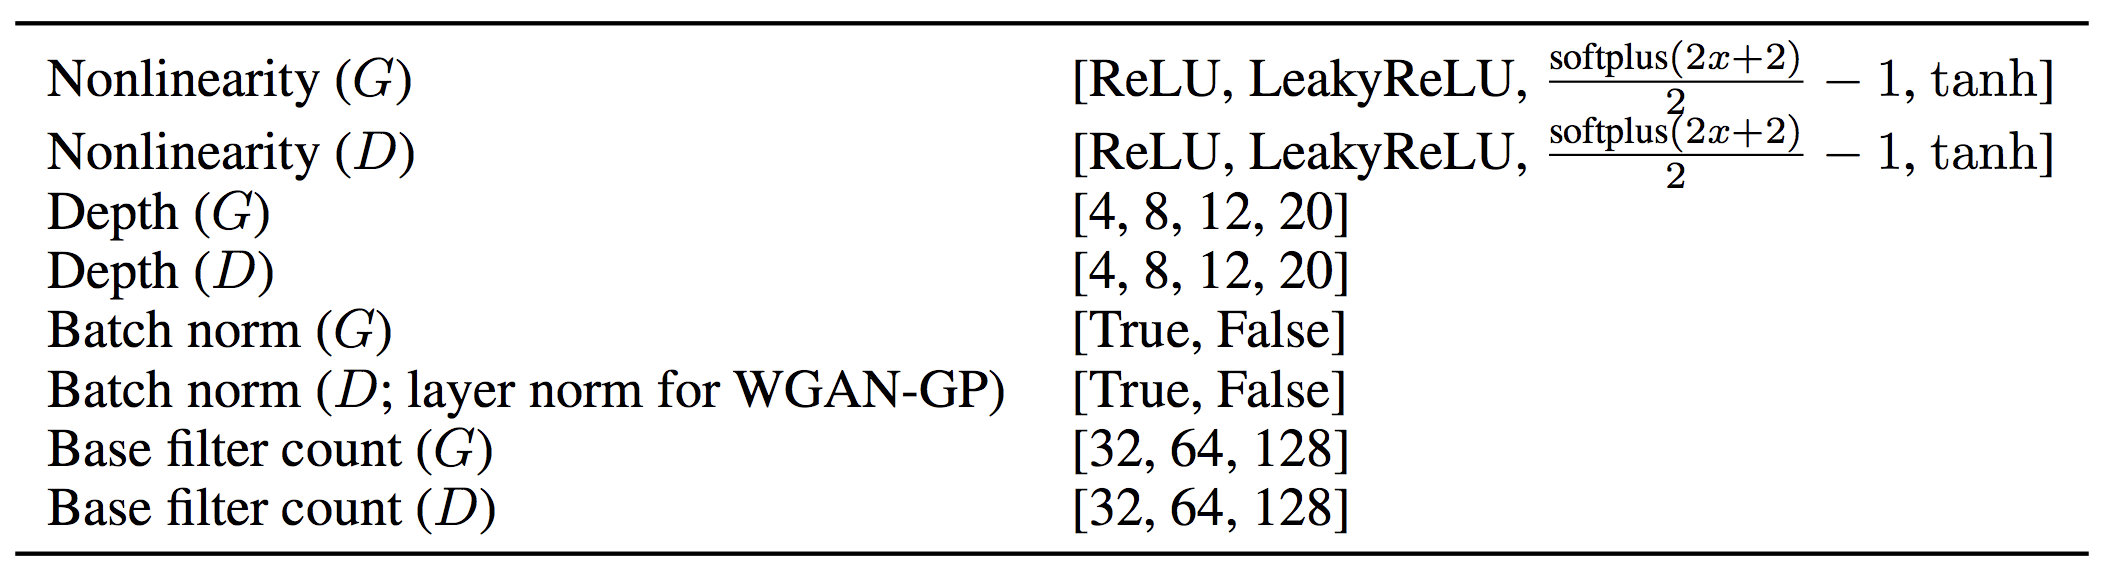
\includegraphics[height=0.8\textheight, width=1.05\textwidth, keepaspectratio]{images/gan/wgan-gp/slide_88_1_img.png}
    \end{figure}
    \begin{figure}
        \centering
        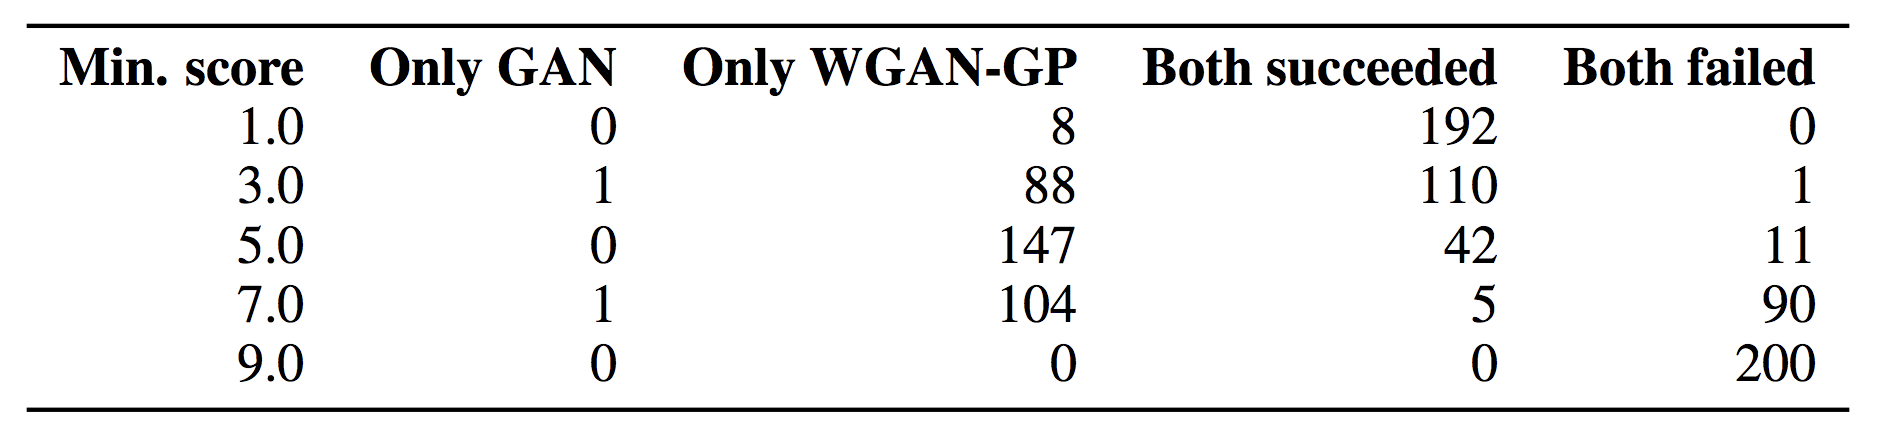
\includegraphics[height=0.8\textheight, width=1.05\textwidth, keepaspectratio]{images/gan/wgan-gp/slide_88_2_img.png}
        \caption*{[Gulrajani et al 2017]}
    \end{figure}

    \framebreak

    \begin{figure}
        \centering
        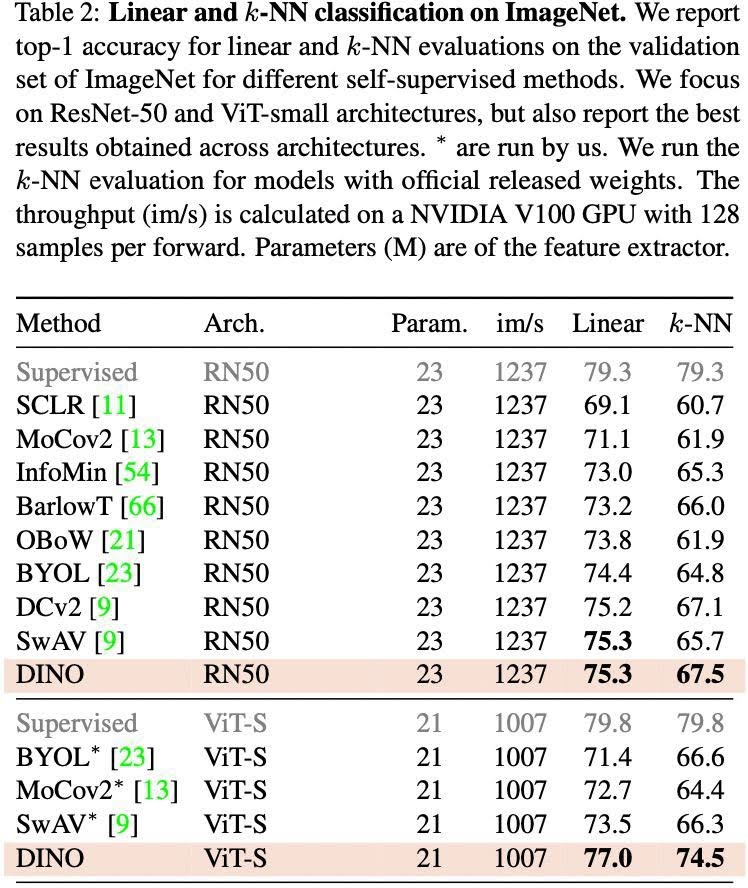
\includegraphics[height=0.85\textheight, width=1.05\textwidth, keepaspectratio]{images/gan/wgan-gp/slide_89_1_img.png}
        \caption*{[Gulrajani et al 2017]}
    \end{figure}
\end{frame}


\begin{frame}[allowframebreaks]{WGAN-GP: High quality samples}
    \begin{figure}
        \centering
        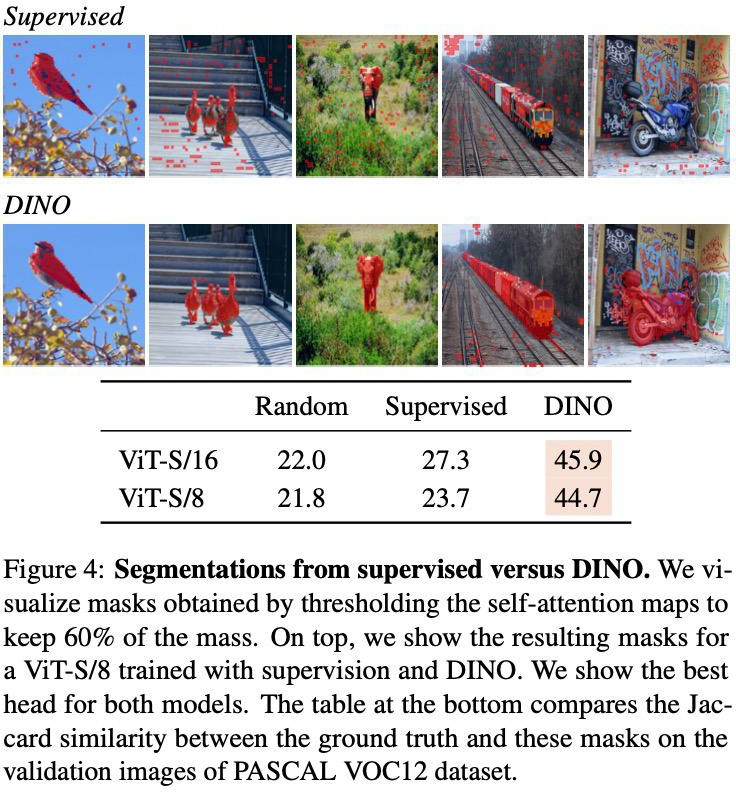
\includegraphics[height=0.8\textheight, width=1.05\textwidth, keepaspectratio]{images/gan/wgan-gp/slide_90_1_img.png}
        \caption*{[Gulrajani et al 2017]}
    \end{figure}

    \framebreak

    \begin{figure}
        \centering
        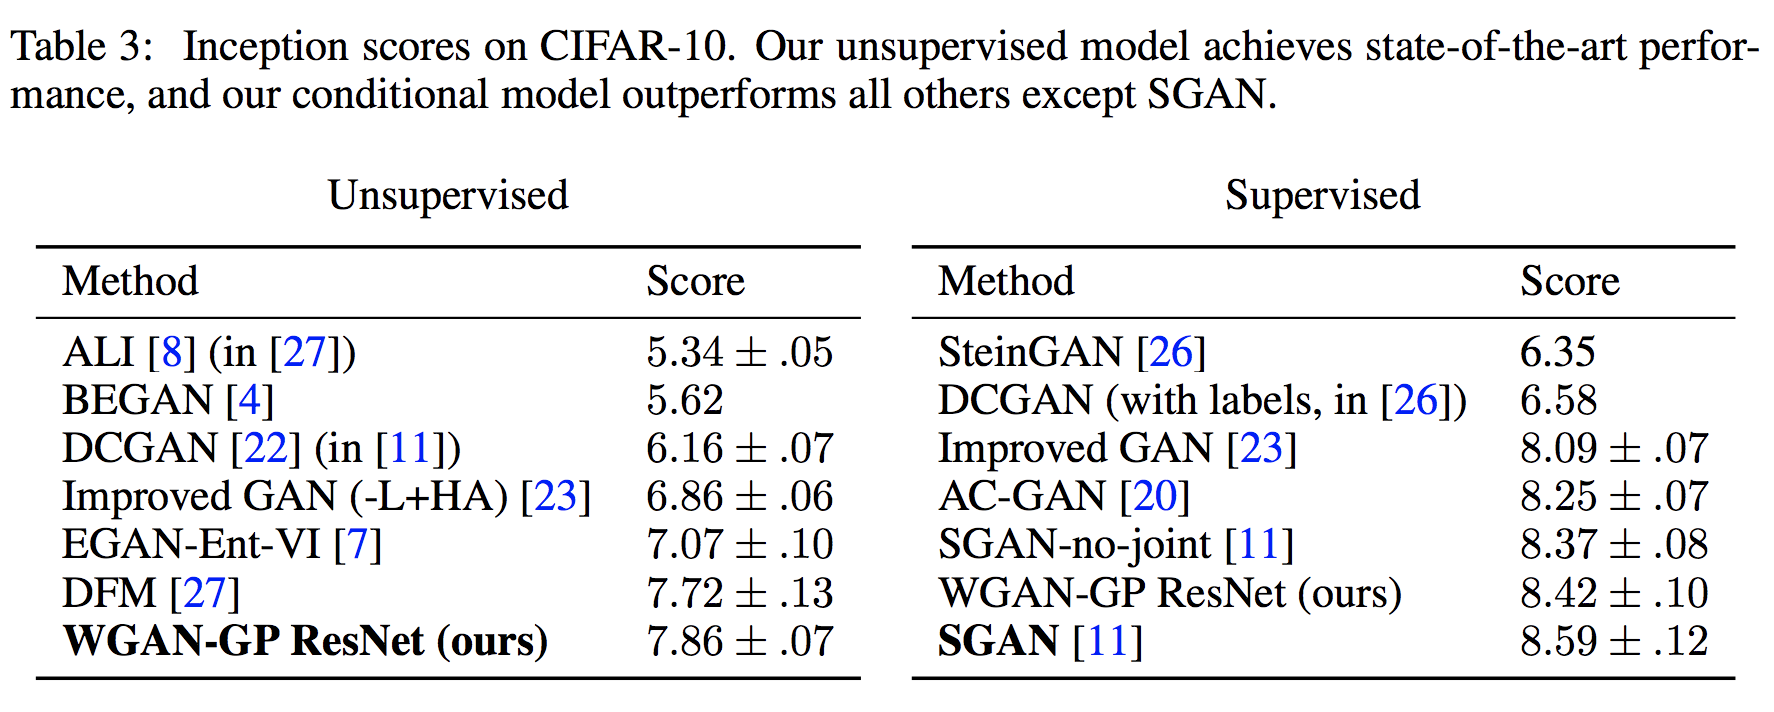
\includegraphics[height=0.8\textheight, width=1.05\textwidth, keepaspectratio]{images/gan/wgan-gp/slide_91_1_img.png}
        \caption*{[Gulrajani et al 2017]}
    \end{figure}
\end{frame}